%\documentclass[pdftex,a4paper]{article}
\documentclass[a4paper]{article}
%%classes: article, report, book, proc, amsproc



%%%%%%%%%%%%%%%%%%%%%%%%
%% Misc

% para acertar os acentos
\usepackage[brazilian]{babel} 
% \usepackage[portuguese]{babel} 
% \usepackage[english]{babel}
\usepackage[T1]{fontenc}
% \usepackage{aeguill}
%\usepackage[latin1]{inputenc}
\usepackage[utf8]{inputenc}
\usepackage{indentfirst}
\usepackage{fullpage}
\usepackage{appendix}
\usepackage{verbatim}
\usepackage{graphicx} %See PDF section
%%%%%%%%%%%%%%%%%%%%%%%%

% %%%%%%%%%%%%%%%%%%%%%%%%
% %% BibTeX !!
% %\usepackage{bibtex}
% \bibliographystyle{mybibtex} % .bst file
% %\bibstyle{prsty} % Choose Phys. Rev. style for bibliography

% %% Natbib
% \usepackage{natbib}
% \bibpunct{[}{]}{;}{a}{,}{,}
% %%%%%%%%%%%%%%%%%%%%%%%%

%%%%%%%%%%%%%%%%%%%%%%%%
%% PDF support

%\usepackage[pdftex]{color,graphicx}
%% Hyper-refs
%\usepackage[pdftex]{hyperref} % for printing
%\usepackage[pdftex,bookmarks,colorlinks]{hyperref} % for screen

%% \newif\ifPDF
%% \ifx\pdfoutput\undefined\PDFfalse
%% \else\ifnum\pdfoutput > 0\PDFtrue
%%      \else\PDFfalse
%%      \fi
%% \fi

%% \ifPDF
%%   \usepackage[T1]{fontenc}
%%   \usepackage{aeguill}
%%   \usepackage[pdftex]{graphicx,color}
%%   \usepackage[pdftex]{hyperref}
%% \else
%%   \usepackage[T1]{fontenc}
%%   \usepackage[dvips]{graphicx}
%%   \usepackage[dvips]{hyperref}
%% \fi

%%%%%%%%%%%%%%%%%%%%%%%%

%%%%%%%%%%%%%%%%%%%%%%%%
%% Math
\usepackage{amsmath,amsfonts,amssymb}
% para usar R de Real do jeito que o povo gosta
%\usepackage{amsfonts} % \mathbb
% para usar as letras frescas como L de Espaco das Transf Lineares
\usepackage{mathrsfs} % \mathscr

% % Theorems' labels, etc.
% \newtheorem{lema}{Lemma}[section] 
% \newtheorem{teor}[lema]{Theorem}
% \newtheorem{defi}[lema]{Definition}
% \newtheorem{prop}[lema]{Proposition}
% \newtheorem{coro}[lema]{Corolary}
% \newtheorem{exem}[lema]{Example}
% \newtheorem{apteor}{Theorem}[chapter]

% Proof commands
% \newcommand{\proofbegin}{\noindent{\bf Proof:} }
% \newcommand{\proofend}{ \hfill $\Box$ \smallskip }

% dt of integrals = \ud t
\newcommand{\ud}{\mathrm{d}}
%%%%%%%%%%%%%%%%%%%%%%%%

\usepackage{url}




%\twocolumn

\author{Felipe Figueiredo}
\title{Consultoria de Análise de Dados para Daisy Lyra (Mestrado Profissional INTO)}
\date{2015}

\begin{document}
\maketitle
\newpage
\tableofcontents
\listoffigures
\listoftables
\newpage
\section{Metodologia utilizada}

(O texto abaixo foi adaptado da versão original do projeto).


A análise descritiva foi apresentada na forma de tabelas os dados observados, expressos pela média, desvio padrão, mediana, amplitude interquartílica (AIQ), mínimo e máximo para dados numéricos (quantitativos) e pela frequência (n) e percentual (\%) para dados categóricos (qualitativos). São apresentados gráficos descritivos das variáveis basais e finais. Ao longo do texto, as variáveis normais foram sumarizadas como média $\pm$ desvio-padrão (DP), e as variáveis não-normais como mediana $\pm$ AIQ.



Foi aplicado o teste de normalidade de Shapiro-Wilks nas variáveis numéricas. A comparação das variáveis basais e finais foi feita com o teste t pareado para variáveis normalmente distribuídas,  e com o teste de Mann-Whitney pareado para variáveis que tiveram a hipótese de normalidade rejeitada. Em todas as análises, foi adotada a  significância de 5\%. As análises estatística foram feitas utilizando o software estatístico R, versão 3.2.2 (\url{https://www.R-project.org}).

\section{Resultados}

\subsection{Estatísticas descritivas}

\subsubsection{Estatísticas}

\begin{table}[!h]
  \centering
  \begin{tabular}{c|ccccc}
    \hline
    Variável& Média (DP) &Mediana (AIQ)&&&\\
    \hline
    \hline
    Vitamina D basal&&&&&\\
    Vitamina D final&&&&&\\
    \hline
    ADP basal &&&&&\\
    ADP final&&&&&\\
    CTX basal &&&&&\\
    CTX final&&&&&\\
    FAO basal &&&&&\\
    FAO final&&&&&\\
    LEP basal &&&&&\\
    LEP final&&&&&\\
    OPG basal &&&&&\\
    OPG final&&&&&\\
    TNF basal &&&&&\\
    TNF final&&&&&\\
    \hline
  \end{tabular}
  \caption[Estatísticas descritivas]{Estatísticas descritivas (terminar de preencher)}
  \label{tab:descritivas}
\end{table}

As estatísticas descritivas das variáveis analisadas estão sumarizadas na tabela \ref{tab:descritivas}\ldots

\begin{itemize}
\item 3 colunas, com cada var por linha, ou uma linha com colunas para basal e final?
\end{itemize}

\subsubsection{Gráficos}

Figuras \ref{fig:vitd-boxplot}, \ref{fig:marcadores-boxplot} mostram as variáveis\ldots

\begin{figure}[!h]
  \centering
  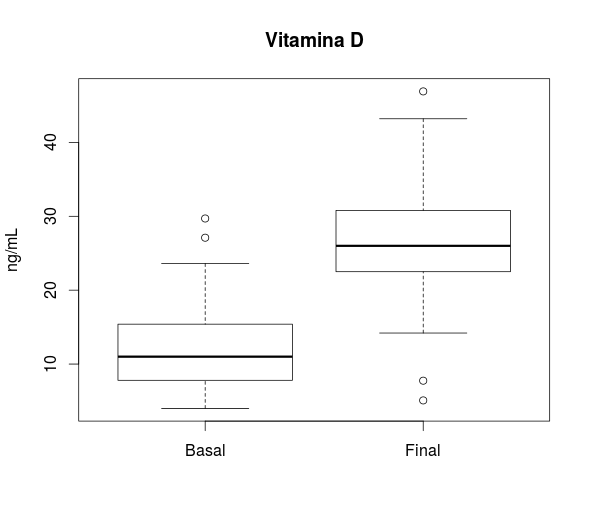
\includegraphics[width=.5\textwidth]{../figuras/vitaminad}
  \caption[Níveis basal e final de vitamina D]{Níveis basal e final de vitamina D. (boxplot: mediana, quartis, outliers)}
  \label{fig:vitd-boxplot}
\end{figure}

\begin{figure}[!h]
  \centering
  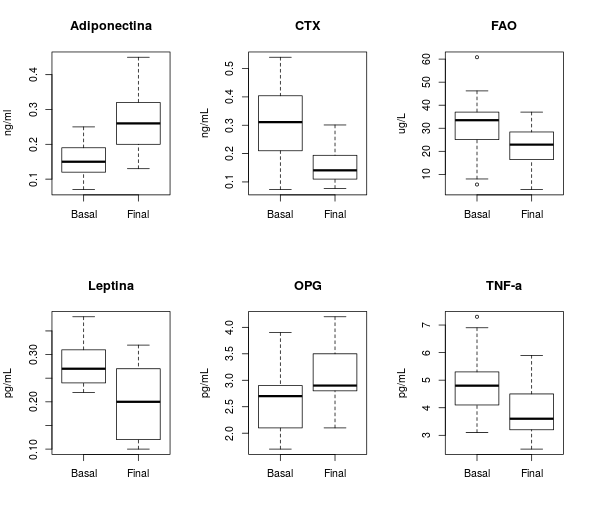
\includegraphics[width=.5\textwidth]{../figuras/boxplots}
  \caption[Níveis basal e final dos marcadores ADP, CTX, FAO, LEP, OPG e TNF]{Níveis basal e final dos marcadores ADP, CTX, FAO, LEP, OPG e TNF (siglas e boxplot: mediana, quartis, outliers)}
  \label{fig:marcadores-boxplot}
\end{figure}

São apresentadas nas figuras \ref{fig:vitd-scatter} e \ref{fig:marcadores-scatter} as retas de melhor ajuste aos 

Os níveis basal e final foram significativamente diferentes, conforme seção \ref{sec:pareados}, e resumidos na tabela \ref{tab:testes-pareados}.


\begin{figure}[!h]
  \centering
  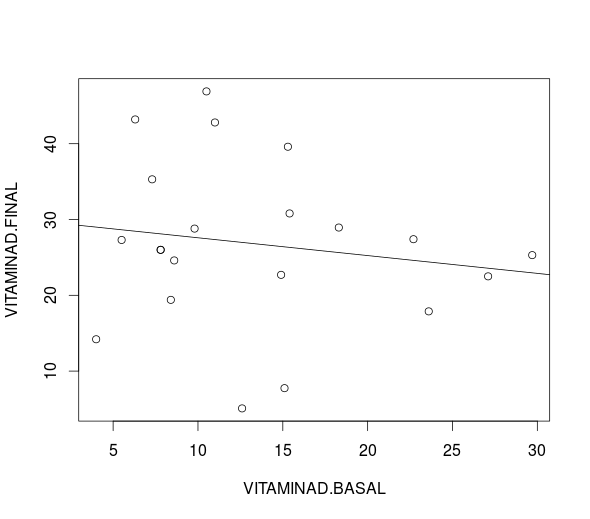
\includegraphics[width=.5\textwidth]{../figuras/vitd-scatter}
  \caption{preencher}
  \label{fig:vitd-scatter}
\end{figure}

\begin{figure}[!h]
  \centering
  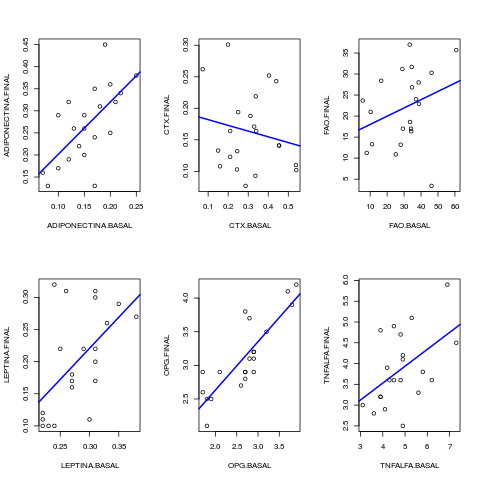
\includegraphics[width=.5\textwidth]{../figuras/scatterplots}
  \caption{preencher}
  \label{fig:marcadores-scatter}
\end{figure}

\begin{itemize}
\item Fazer histogramas das variáveis.
\end{itemize}

\newpage
\subsection{Normalidade}

P: textual ou tabela?

\newpage
\subsection{Testes pareados}
\label{sec:pareados}

\begin{table}[!h]
  \centering
  \begin{tabular}{c|cc|c}
    \hline
    Variável&Valor basal mediano (AIQ) &Valor final mediano (AIQ) &p-valor\\
    \hline
    \hline
    Vitamina D&&&\\
\hline
    ADP&&&\\
    CTX&&&\\
    FAO&&&\\
    LEP&&&\\
    OPG&&&\\
    TNF&&&\\
    \hline
  \end{tabular}
  \caption[Diferenças entre os valores basal e final dos marcadores]{Diferenças entre os valores basal e final dos marcadores. Siglas... (terminar). Mann-Whitney pareado}
  \label{tab:testes-pareados}
\end{table}

\end{document}
